\documentclass[tikz,border=5pt]{standalone}
\usetikzlibrary{calc}
\begin{document}
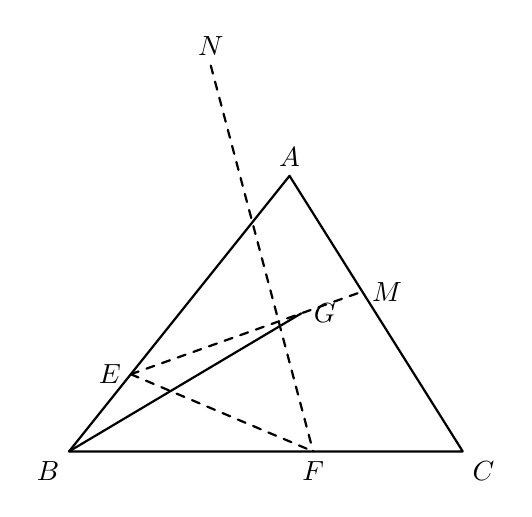
\begin{tikzpicture}[line cap=round,line join=round]
  % main triangle ABC
  \coordinate (B) at (0,0);
  \coordinate (C) at (5,0);
  \coordinate (A) at (2.8,3.5);
  \draw[thick] (B) -- (C) -- (A) -- cycle;

  % points on edges
  \coordinate (E) at ($(B)!0.28!(A)$);
  \coordinate (M) at ($(A)!0.42!(C)$);
  \coordinate (F) at ($(B)!0.62!(C)$);
  \coordinate (N) at (1.8,4.9);

  % intersection point G on dashed line AF
  \coordinate (G) at (intersection of E--M and A--F);

  % dashed construction lines
  \draw[thick,dashed] (N) -- (F);
  \draw[thick,dashed] (E) -- (M);
  \draw[thick,dashed] (E) -- (F);

  % new solid segment BG
  \draw[thick] (B) -- (G);

  % labels
  \node[below left] at (B) {$B$};
  \node[below right] at (C) {$C$};
  \node[above] at (A) {$A$};
  \node[left] at (E) {$E$};
  \node[right] at (M) {$M$};
  \node[below] at (F) {$F$};
  \node[above] at (N) {$N$};
  \node[right=1pt] at (G) {$G$};
\end{tikzpicture}
\end{document}
